\documentclass[10pt]{beamer}

\usepackage{hyperref}
\hypersetup{
    colorlinks=true,
    linkcolor=black,
    filecolor=black,
    urlcolor=blue,
    citecolor=black
}


% Add these packages in the preamble
\usepackage{listings}
\usepackage{xcolor}

% Add this styling configuration
\lstdefinestyle{mystyle}{
    backgroundcolor=\color{gray!10},
    basicstyle=\ttfamily\small,
    breakatwhitespace=false,
    breaklines=true,
    captionpos=b,
    commentstyle=\color{green!60!black},
    keywordstyle=\color{blue},
    stringstyle=\color{red},
    showspaces=false,
    showstringspaces=false,
    showtabs=false,
    tabsize=2,
    frame=single
}
\lstset{style=mystyle}




\usepackage{verbatim}
\usetheme[progressbar=foot]{metropolis}
\usepackage{appendixnumberbeamer}

\usepackage{booktabs}
\usepackage[scale=2]{ccicons}

\usepackage{pgfplots}
\usepgfplotslibrary{dateplot}

\usepackage{xspace}
\usepackage{xcolor}

\usepackage{pifont}
\newcommand{\cmark}{\textcolor{green!70!black}{\ding{51}}} % check mark
\newcommand{\xmark}{\textcolor{red}{\ding{55}}}             % cross mark

\DeclareMathOperator{\stdev}{stdev}
\DeclareMathOperator{\var}{var}
\DeclareMathOperator{\cov}{cov}
\DeclareMathOperator{\corr}{corr}
\DeclareMathOperator{\prob}{prob}
\DeclareMathOperator{\n}{n}
\DeclareMathOperator{\N}{N}
\DeclareMathOperator{\Cov}{Cov}

\newcommand{\D}{\mathrm{d}}
\newcommand{\E}{\mathrm{e}}
\newcommand{\mye}{\ensuremath{\mathsf{E}}}
\newcommand{\myreal}{\ensuremath{\mathbb{R}}}

\setbeamertemplate{frame footer}{MGMT 675}


\setbeamertemplate{title page}{
  \begin{centering}
    \begin{beamercolorbox}[sep=8pt,center]{title}
      \usebeamerfont{title}\inserttitle\par%
      \ifx\insertsubtitle\@empty%
      \else%
        \vskip0.25em%
        {\usebeamerfont{subtitle}\usebeamercolor[fg]{subtitle}\insertsubtitle\par}%
      \fi%     
    \end{beamercolorbox}%
    \vfill
    \begin{beamercolorbox}[sep=8pt,center]{date}
      \usebeamerfont{date}\insertdate
    \end{beamercolorbox}
    \vskip0.5em
    {\usebeamercolor[fg]{titlegraphic}\inserttitlegraphic\par}
  \end{centering}
}


\title{AI Overview}
\subtitle{MGMT 675: AI-Assisted Financial Analysis}
\titlegraphic{
\includegraphics[height=1cm]{../docs/RiceBusiness-transparent-logo-sm.png}}
\date{}
\begin{document}

\begin{frame}[plain]
\titlepage
\end{frame}

\section{API Calls}
\begin{frame}{Creating an App that Makes API Calls}
\begin{itemize}
    \item Get an API key from OpenAI or other LLM provider
\item Generate code that sends a prompt to an AI and gets a response.  API key should be included in code to authorize (for billing).
\item Or create an interface that allows the user to formulate a prompt.  Your code may expand the prompt to include whatever information you want to provide to the LLM.
\item Or send your own prompt and allow users to send prompts.
\end{itemize}
\end{frame}

\begin{frame}{Examples}
    \begin{itemize}
        \item Julius prompt: build a Streamlit app that scrapes the headlines from \textit{The Guardian} website, sends them to ChatGPT 4o using my API key, and returns a summary of the headlines and an assessment of the sentiment of the headlines.
      \begin{itemize}
        \item After deployment: \href{https://mgmt675-app-kbhft94zmjfhfjqbdq9csf.streamlit.app/}{Streamlit app with API call built by Julius}
        \end{itemize}
        \item Replit prompt: same as Julius prompt + provide a chat interface that allows the user to ask further questions about the headlines.
        \begin{itemize}
        \item Deployed directly from Replit: \href{https://guardian-pulse-kerryback.replit.app/}{Replit app with API call}
        \end{itemize}
        \item Build apps with \href{https://zapier.com/blog/categories/zapier-automation/}{Zapier}
    \end{itemize}
    \end{frame}

    % Replace your verbatim block with this:
\begin{frame}[fragile]{Python code for API call}
    \begin{lstlisting}[language=Python]
import openai
# [input openai_api_key]
client = openai.OpenAI(api_key=openai_api_key)
prompt = "Here are today's headlines"
# [then include the scraped headlines]
prompt += "Based on these headlines, ..."
response = client.chat.completions.create(
    model="gpt-4o",
    messages=[
        {"role": "system", "content": "You are a helpful assistant that analyzes news headlines."},
        {"role": "user", "content": prompt}
    ]
)
    \end{lstlisting}
\end{frame}

   

    \begin{frame}{API-based Apps vs AI Agents}

        From ChatGPT:

        \begin{table}[h!]
        \centering
        \renewcommand{\arraystretch}{1.3}
        \begin{tabular}{|l|c|c|}
        \hline
        \textbf{Feature} & \textbf{API-based App} & \textbf{AI Agent} \\
        \hline
        Autonomy & \xmark{} Only reacts & \cmark{} Acts independently \\
        Goal-Oriented & \xmark{} Task-based & \cmark{} Goal-driven \\
        Adaptability & \xmark{} Predefined logic & \cmark{} Can adapt behavior \\
        Tool Use & \cmark{} Manual calls & \cmark{} Chooses tools as needed \\
        Memory & \xmark{} Usually none & \cmark{} May have memory \\
        Intelligence Level & \xmark{} Fixed logic & \cmark{} Planning \& reasoning \\
        \hline
        \end{tabular}
        \end{table}

        
        \end{frame}

\section{Some Chatbots}

\begin{frame}{Chatbots}
    \begin{itemize}
     \item ChatGPT, Gemini, Claude, Perplexity (try ChatGPT Deep Research)
     \item \href{https://openai.com/index/introducing-gpts/}{Custom GPTs}
    \item \href{https://notebooklm.google/}{Google NotebookLM}
    \begin{itemize}
        \item Notebook = collection of sources (text, images, etc.)
        \item Can ask questions about the sources
        \item Can create audio ("podcast") from the sources
    \item Example: \href{https://hai.stanford.edu/ai-index/2025-ai-index-report}{Stanford AI Report 2025}
    \item \href{https://notebooklm.google.com/notebook/83e22c17-71bf-4bb2-a803-294ffe11d365/audio}{NotebookLM podcast version} also at \href{https://www.dropbox.com/scl/fi/ui3b7et1mi575b947n11s/Stanford_AI_Report_2025.wav?rlkey=dpfb7i75uk1yhecn668bzwp2w&dl=1}{this link}
    \end{itemize}
    \item \href{https://openrouter.ai/}{OpenRouter} provides access to many LLMs.  Use your own API keys for paid LLMs or use free LLMs.
        \end{itemize}
    \end{frame}

\section{Language Models}

\begin{frame}{Tokenization, Embedding, and Prediction}
    \begin{enumerate}
        \item Tokenization: break text into tokens (words, characters, or subwords). Example: unhappiness $\rightarrow$ [un, happy, ness]
        \item Embedding: assign each token to a vector (list of numbers)
        \vspace{1em}
    \begin{center}
       \alert{Tokenization $+$ Embedding $\rightarrow$ text translated into sequence of vectors}
        \end{center}   \vspace{1em}
        \item Prediction problem:
        given a sequence of vectors, predict the next vector
        \vspace{1em}
        \begin{center} \alert{Embedding $+$ Prediction optimized jointly by machine learning} \end{center}
    \end{enumerate}
\end{frame}


\begin{frame}{Example: GPT-3}
    \begin{itemize}
        \item Tokenization: use 50,257 tokens
        \item Embedding: each token assigned to a vector of 12,288 numbers. 
        \begin{itemize}
        \item 50,257 tokens $\times$ 12,288 numbers per token $=$ 617 million numbers (parameters)
        \end{itemize}
        \item Prediction: Use sequence of 2,048 prior tokens to predict next token.
        \vspace{-1em}
        \begin{itemize}
        \item 2,048 tokens is 2,048 $\times$ 12,288 = 25 million numbers 
        \item Used to predict next token, which is 
        12,288 numbers
        \item So, predict $y$ from $x$ with 25 million $x$ variables and 12,288 $y$ variables (per observation)
        \end{itemize}
    \end{itemize}
\end{frame}

\begin{frame}{Summary of GPT-3}
    \begin{center}
    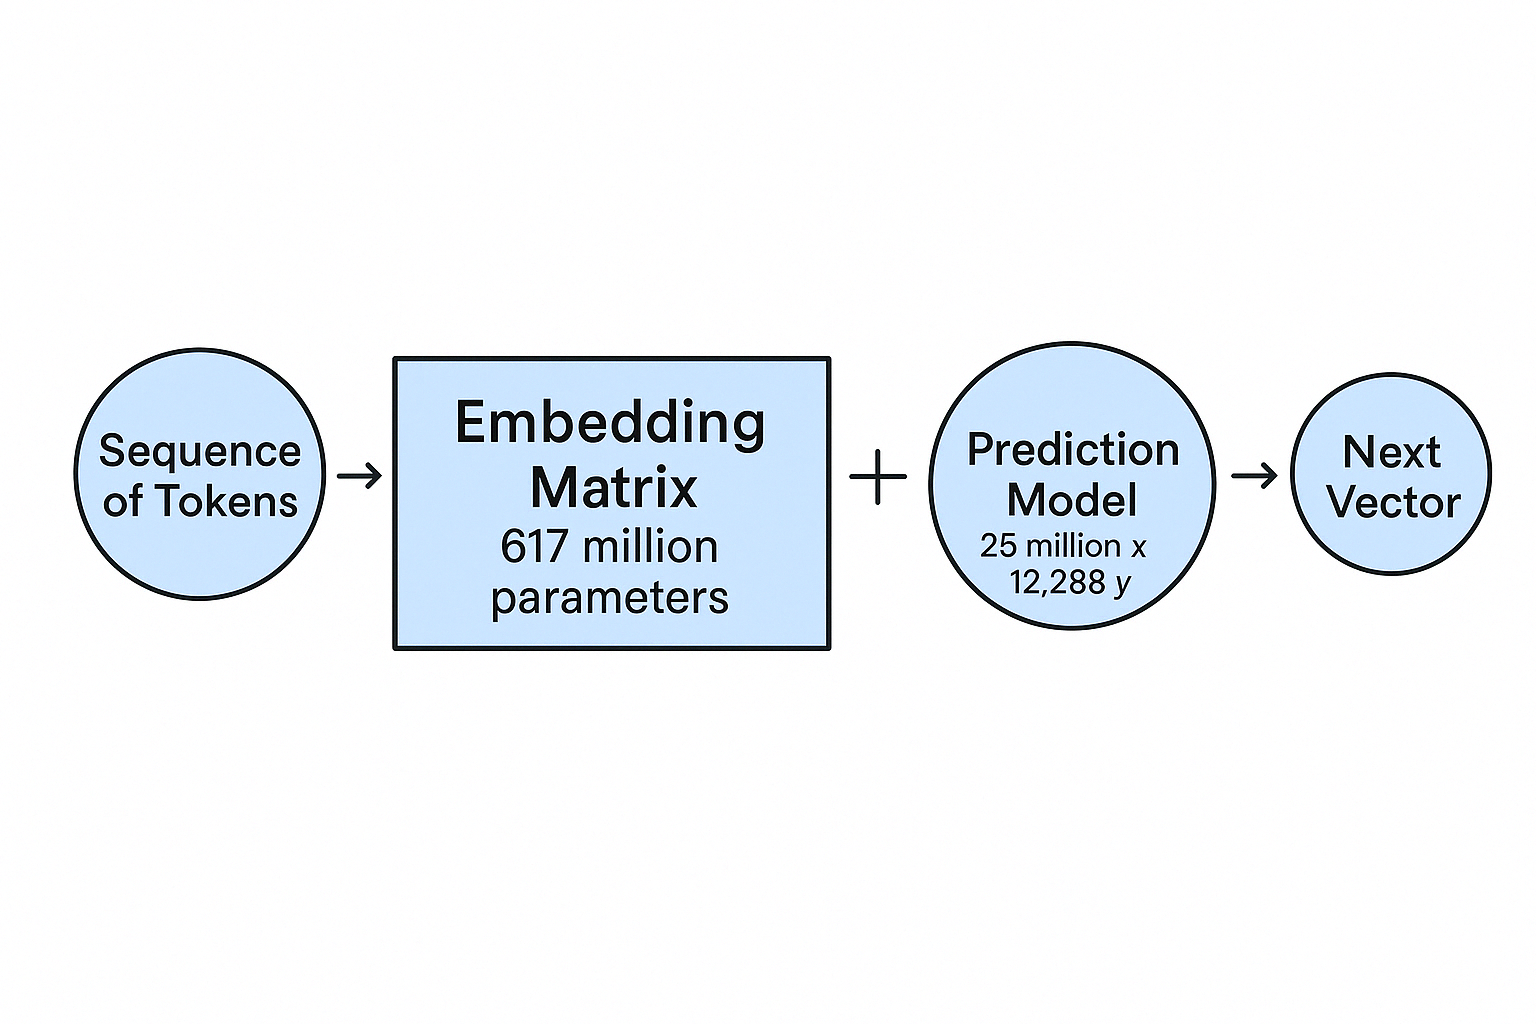
\includegraphics[width=0.8\textwidth]{../images/gpt5.png}
    \end{center}
\end{frame}

\begin{frame}{GPT-3.5 Turbo Embeddings}
    \begin{itemize}
        \item Can get vector embeddings of tokens from Chat GPT 3.5 Turbo by API calls 
        \item Vectors are 1,536 numbers long
        \item \href{https://mgmt675-2025/assets/embeddings.xlsx}{Excel file} with vector embeddings of king, queen, woman, and man from ChatGPT 3.5 Turbo
        \item Famous example: can add and subtract vectors and king $+$ woman $-$ man $\approx$ queen
    \end{itemize}
\end{frame}

\section{Neural Networks (Prediction Model)}

\begin{frame}{History of Neural Networks}
    \begin{description}
      \item[1943:] McCulloch \& Pitts propose a binary threshold model of neurons.
      \item[1958:] Perceptron introduced by Frank Rosenblatt 
      \item[1986:] Backpropagation popularized by Rumelhart, Hinton, \& Williams enables training of multilayer networks.
      \item[1990s:] Recurrent Neural Networks (RNNs) and Convolutional Neural Networks (CNNs) gain traction.
      \item[1997:] Long Short-Term Memory (LSTM) addresses RNN vanishing gradient issues (Hochreiter \& Schmidhuber).
      \item[2012:] AlexNet wins ImageNet, marking deep learning's breakthrough.
      \item[2017:] \alert{Transformers introduced} --- Vaswani et al.\ publish \emph{Attention Is All You Need}, replacing recurrence with self-attention.
      \item[2020s:] Transformer variants dominate NLP and spread to vision and multi-modal models. GPT = Generative Pre-trained Transformer.
   \end{description}
\end{frame}

\begin{frame}{Multi-Layer Perceptrons}
    \begin{itemize}
        \item A multi-layer perceptron (MLP) consists of ``neurons'' arranged in layers.
        \item A neuron is a mathematical function. It takes inputs $x_1, \ldots, x_n$, calculates a function $y=f(x_1, \ldots, x_n)$ and passes $y$ to the neurons in the next level.
        \item Standard function (ReLU) for hidden layers is 
        $$y = \begin{cases}\alpha+\beta_1x_1 + \cdots + \beta_nx_n & \text{if positive} \\ 0 & \text{otherwise}\end{cases}$$
        \begin{itemize}
            \item First layer (input layer) $=$ inputs (features).
            \item ``Hidden layers'' take inputs from previous layer and pass output to next layer.
            \item Last layer (output layer) has one neuron for each output.
        \end{itemize}
    \end{itemize}
    \end{frame}
    
    \begin{frame}{Illustration}
 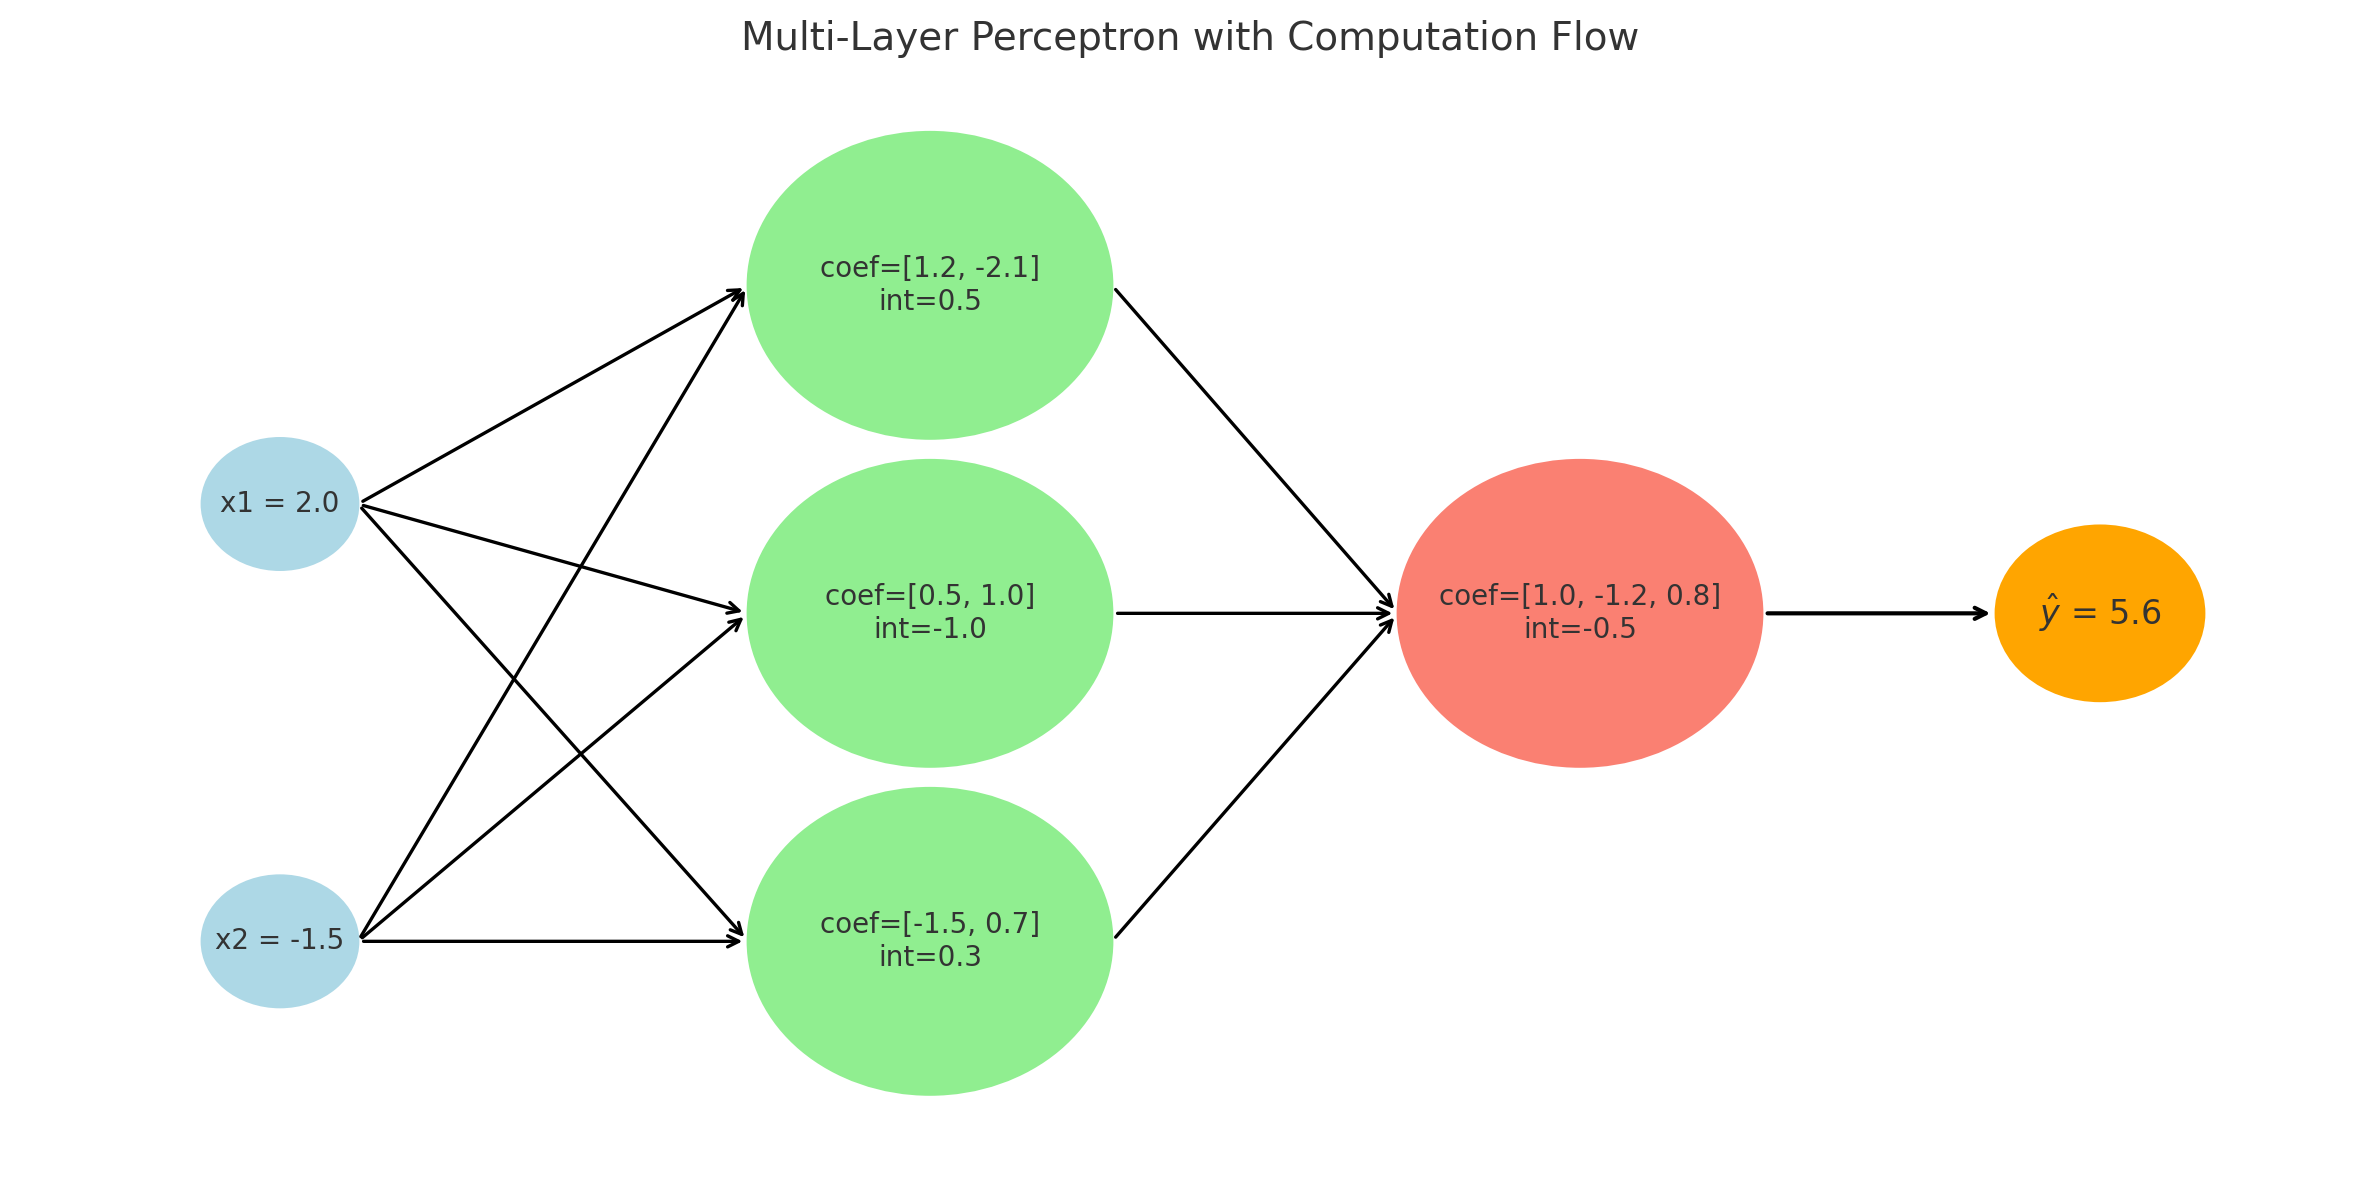
\includegraphics[width=1.15\textwidth]{../images/net2.png}

\end{frame}

\begin{frame}{Hidden Layer Computations}
    Inputs $x_1 = 2.0$, $x_2 = -1.5$
    
    \begin{description}
    \item[Neuron 1] $\alpha = 0.5$, $\beta_1 = 1.2$, $\beta_2 = -2.1$
    \begin{align*}
    h_1 &= \text{ReLU}(0.5 + 1.2 \cdot 2.0 + (-2.1) \cdot (-1.5)) \\
            &= \text{ReLU}(6.05) = 6.05
    \end{align*}
      
     \item[Neuron 2] $\alpha = -1.0$, $\beta_1 = 0.5$, $\beta_2 = 1.0$
    \begin{align*}
    h_2 &= \text{ReLU}(-1.0 + 0.5 \cdot 2.0 + 1.0 \cdot (-1.5)) \\
        &= \text{ReLU}(-1.5) = 0
    \end{align*}

    \item[Neuron 3] $\alpha = 0.3$, $\beta_1 = -1.5$, $\beta_2 = 0.7$
    \begin{align*}
    h_3 &= \text{ReLU}(0.3 + (-1.5) \cdot 2.0 + 0.7 \cdot (-1.5)) \\
        &= \text{ReLU}(-3.75) = 0
    \end{align*}
    \end{description}
    \end{frame}
    
    \begin{frame}{Output Computation}
         $\alpha = -0.5$, $\beta_1 = 1.0$, $\beta_2 = -1.2$, $\beta_3 = 0.8$
    \begin{align*}
    \hat{y} &= -0.5 + 1.0 \cdot h_1 + (-1.2) \cdot h_2 + 0.8 \cdot h_3 \\
            &= -0.5 + 6.05 + 0 + 0 = \boxed{5.55}
    \end{align*}
    \end{frame}
    
\end{document}

